% this file is called up by thesis.tex
% content in this file will be fed into the main document

\chapter{Implementation} % top level followed by section, subsection


% ----------------------- paths to graphics ------------------------

% change according to folder and file names
\ifpdf
    \graphicspath{{7/figures/PNG/}{7/figures/PDF/}{7/figures/}}
\else
    \graphicspath{{7/figures/EPS/}{7/figures/}}
\fi

\section{OpenCSD}

In this section we describe the tools and techniques used with the OpenCSD
framework, detail modules with their respective functionality and show the
external dependencies as well as internal relationships of these modules. 
Followed by, sections on filesystem and offloading implementation details.

\subsection{Framework}

Firstly, OpenCSD consist of many external dependencies, most prominently
\textit{Storage Performance Development Kit} (SPDK) \cite{spdk} and uBPF
\cite{ubpf}. These technolgies are used as userspace NVMe SSD driver and as
virtual machine for the eBPF ISA respectively. Reusing as many as pre-existing
technologies as possible increases the change of familiarity aiding ease of use.
More prominently, these existing technologies dramatically lower the amount of
development effort required to create the prototype. However, our design
requirements demand these dependencies be installed in an isolated way. To do
this OpenCSD configures an isolated build environment with dependencies made
available through an environment file. Moreover, this file configures variables
such as \textit{PATH} and \textit{LD\_LIBRARY\_PATH}. In addition, OpenCSD
offers a QEMU installation and accompanying qcow image to emulate a ZNS SSDs.
This is to overcome the limited availability of these SSDs as stated in the
design requirements. However, the use of QEMU for ZNS SSDs is entirely optional.
Finally, CMake \cite{cmake} is used to orchestrate the installation of
dependencies as well as the compilation of binary targets. Due to limitations it
is advised to rerun CMake after each make command, as this  prevents unnecessary
recompilation of external dependencies \footnotemark[10]. The combination of this
isolated dependencies environment managed through CMake with the ability to use
QEMU for ZNS SSDs emulation is ideal to minimize the complexity as exposed to
users of OpenCSD.

\footnotetext[10]{Due to limitations in the evaluation of file presence
conditions which are not reevaluated when executing the generated makefile.}

As said OpenCSD is comprised of modules using a component architecture.
Additionally, Each module is compiled as a static or shared library to reduce
coupling. This creates an explicit nature of exchanging information between
linked libraries that allows to identify feasibility problems at an early stage.
This is opposed to potentially only identifying such issues when creating a
first hardware prototype. A trivial example of such infeasibilities would be
using shared memory mutexes to synchronize filesystem and CSx kernel behaviour.
Several modules are solely an interface with subsequent modules being one or
more concrete implemenations of these interfaces. These module based interfaces
with loose coupling allow for simplified replacement of technologies.

\subsubsection{Modules}

The overall modules of OpenCSD are shown in figure
\ref{figure:moduledependencies} along with any external or internal
dependencies. In addition, we briefly describe the functionality of each module.
Finally, at the end of this subsection we describe the three most prominent
modules of OpenCSD.

% Diagram with overview of different modules and their used as well as
% relationships. Also show integration of open-source technologies.

\begin{figure}
    \centering
	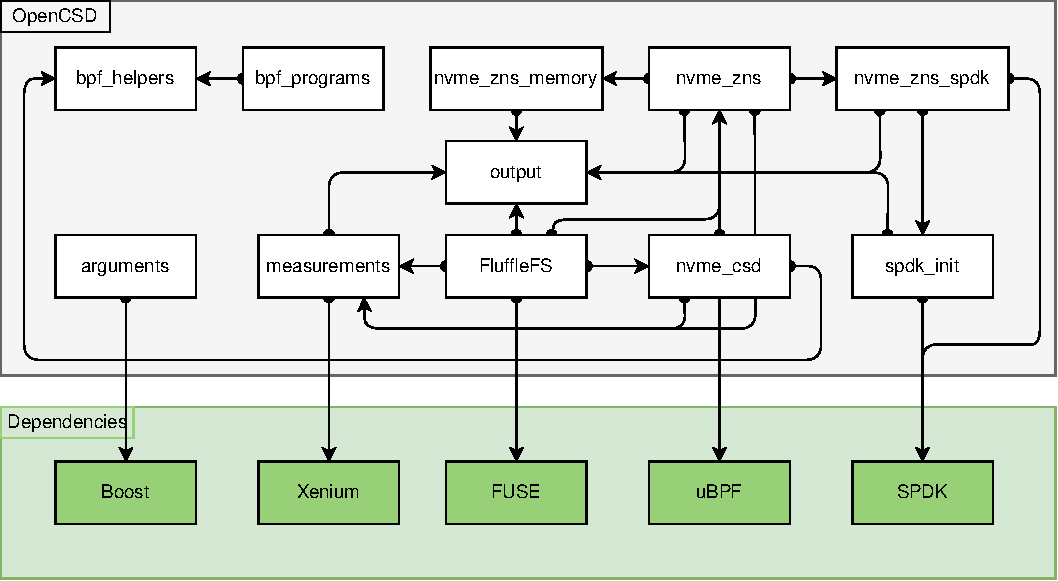
\includegraphics[width=1\textwidth]{resources/images/module-dependencies.pdf}
	\caption{Overview of all OpenCSD components and their depends-on relations}
    % \includesvg[width=0.6\columnwidth]{resources/images/module-dependencies}
    \label{figure:moduledependencies}
\end{figure}

\begin{itemize}
    \item output - Manages stdout and stderr output to the console by
    registering namespaces and providing a variety of log levels.
    \item arguments - Parses command line arguments and splits these into parts
    that can be passed to other modules in a decoupled nature. 
    \item measurements - Low overhead performance instrumentation for functions
    separated by namespaces using high performance lockless unbounded queue
    \cite{Michael1996SimpleFA}.
    \item spdk\_init - Collection of helpers to perform SPDK initialization and
    select ZNS suppporting NVMe namespace.
    \item nvme\_zns - NVMe interface to perform ZNS operations read, write and
    reset. To be used by FluffleFS for decoupled I/O operations.
    \item nvme\_zns\_memory - Memory backed implementation of nvme\_zns
    interface.
    \item nvme\_zns\_spdk - SPDK backed implementation of nvme\_zns interface
    \item nvme\_csd - Simulated extension to the PCIe NVMe protocol that allows
    to perform CSx operations. Execution of kernels is handled through uBPF.
    Utilizes instance of nvme\_zns to perform actual I/O operations performed by
    kernel.
    \item bpf\_helpers - Collection of headers that define the eBPF ABI
    supported for CSx kernels. ABI to be implemented by device vendor
    or in this case nvme\_csd for simulation. The ABI is filesystem agnostic.
    \item bpf\_programs - Collection of eBPF programs linked at runtime for
    previous ZCSD \cite{lukken2021zcsd} prototype.
    \item FluffleFs - FUSE LFS supporting in-memory snapshots to achieve
    multi-user tenancy with concurrent regular and offloaded filesystem access.
    Utilizes, nvme\_zns and nvme\_csd to achieve functionality.
\end{itemize}

Out of these components nvme\_csd, bpf\_helpers and FluffleFS are the most
essential. They simulate the required changes that would realize such an
architecture.

In short nvme\_csd contains functions that should be made part of a new NVMe
command set and namespace \cite{nvme-command} similar to how ZNS was introduced.
Currently, the functions are overly simplified so there is no use of the actual
command layout as well as lack of queue submissions and completion commands. We
feel the concepts of implementing these are well understood and would not
contribute to the scientific value of this work while introducing substantial
additional complexity.

bpf\_helpers contains the ABI exposed to the eBPF kernels. An ABI is different
from an API in that the functions it defines cannot be found in segments of
code, either included statically or through a shared library. Instead it uses
an ISA specific instruction that can be called with a set of arguments, the
arguments matching the function signature. Alternatively, should the ISA not
have a specific \textit{call} instruction, interrupt requests can be used to
achieve the same functionality. Upon calling the control flow is returned to
the operating system or in our case uBPF where the functions behavior is
implemented. The result is that an ABI allows to define functionality with
vendor agnostic implementations, similar to POSIX for operating systems. It
should be noted that ISAs typically have a hard limit on the number of arguments
that can be supported, in the case of eBPF this is five arguments. Lastly, is
FluffleFS which is described in the next section in detail.

Out of all modules only nvme\_zns has been given an abstract interface so the
underlying technologies can be easily replaced. However, we argue the design
requirements are still met as there are virtually no replacements for
technologies used in other modules such as uBPF and FUSE\footnotemark[11].
In addition, we feel it would have beneign benefits to create abstract
interfaces of the C++ STL. Our solution allows for replacing technologies with
readily available alternatives without creating unnecessary interfaces.

\footnotetext[11]{While alternative technolgies to implement filesystems exist
none of them are in userspace. As a result we argue there is no alternative to
FUSE.}

\subsection{Filesystem}

This section describes the filesystem implementation and how it meets the design
requirements. In addition, it describes how data is layed out on the drive as
well as how state is represented in memory. Our implementation borrows heavily
from F2FS \cite{Lee2015F2FSAN} a filesystem already optimized for flash storage.
In addition, F2FS is a LFS as per the design requirements. However, FluffleFS is
written directly for ZNS since it only uses \textit{append}, \textit{read} and
\textit{reset} NVMe commands. While this might seem like a limitation the
decoupled interfaces allow to easily create an emulated ZNS device using a
regular block device.

To describe the filesystem implementation further it is first categorized into
four topics. Firstly, we describe the layout on the drive with high level parts
and data structures expanded to fit onto individual sectors. Secondly, the
in memory representation of filesystem data is described as well as how these
translate to data on the drive. Third, the operational rules for most filesystem
operations are described such as when a file exists or not. Lastly, the
concurrency model of FluffleFS is described as well as some of the concurrency
limitations.

\subsubsection{Layout}

We briefly reintroduce some fundamental terminology for this section. A ZNS
device consist of $\{0,1,...,n-1\}$ zones each with $\{0,1,...,s-1\}$ sectors
where $n$ and $s$ are the number of zones and sectors, respectively. For each of
these zones ZNS can define a sector data limit of $l_{n} < s$. Any sector above
and including $l_{n}$ will be unwriteable for that zone. For simplicity we
assume that $l_{0} = \{l_{1},...,l_{n-1}\}$. Data is appended within each zone
on a per sector basis until the zone is full. To achieve this each of these
zones internally maintains a write-pointer that keeps track of up to which
sector data is written. This information can be queried, however, this process
is reasonably expensive. Unlike regular block devices this write-pointer
information allows to identify reads that would return garbage data from an
unwritten sector. We describe reads to such locations as encountering a
\textit{hole}. Finally, zones must be erased as entire unit at a time.

Beyond ZNS, FluffleFS uses on drive and in-memory datatsructures with some
translation between those. All FluffleFs datastructures on drive are scaled to
fit neatly into a single sector. This scaling of datastructures to fit in
sectors is dynamic but FluffleFS has to be recompiled to work with a different
sector size. Typically when referring data on the drive this is expressed in
terms of \textit{blocks}. Within FluffleFS a block will always be of equal size
to a sector. Just like ZNS, FluffleFS also keeps track of several pointers.
These are write-pointers just like ZNS does itself. More importantly are
wraparound-pointers that allow to use linear drive space as circular contiguous
space. Given this terminology we can now describe the filesystem layout.

In a very high level overview the data layout of FluffleFS is spraid across
three parts. These are a fixed zone, random zone and log zone. These names are
adopted from F2FS and have no relation to ZNS zones. In addition, it should be
noted that the random zone unlike F2FS does not require random writes and has
been adopted to be append only as well.

Firstly the fixed and random zone are explained separely from the log zone.
Their high level layout is shown in figure \ref{figure:flufflelayout}. This high
level layout shows the data in terms of entire zones indexed from ${0,...,n-1}$.
In later more detailed sections individual sectors and their datastructures
are described.

To simplify the filesystem and its management the data in a sector is always
limited to one specific type of datastructure. In addition, the fixed zones
limit the types of datastructure to a single one for the entire zone.

\begin{figure}[h!]
    \centering
	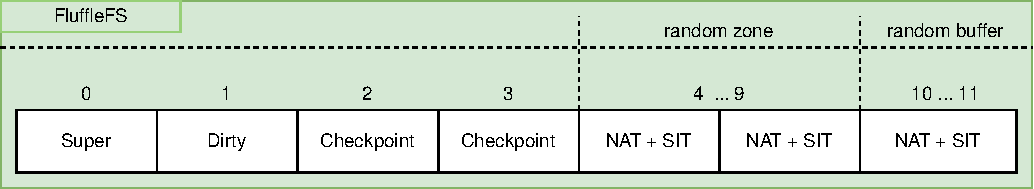
\includegraphics[width=1\textwidth]{resources/images/fluffle-layout.pdf}
	\caption{Fixed and Random zone layouts of FluffleFS.}
    % \includesvg[width=0.6\columnwidth]{resources/images/module-dependencies}
    \label{figure:flufflelayout}
\end{figure}

Consider the fixed zones as depicted in figure \ref{figure:flufflelayout}. In
this region the drive layout distinquishes between three different
datastructures the first two occupying an entire zone.

Firstly, the superblock identifies the filesystem using a magic cookie. In
addition, it remembers the number of zones, sectors and size of sectors the
filesystem should occupy. This metadata allows to identify if the partition was
resized. The superblock is written upon filesystem creation and in principle
never changed. The implication is that the filesystem can not cope with resizing
partitions.

Secondly, the dirtyblock keeps track of filesystem opening and shutdown. The 
block is written upon opening the filesystem and removed once closed completely.
Other datastructures in combination with the dirtyblock allow to identify and
recover from unclean shutdowns.

Lastly, FluffleFS keeps track of checkpoints across two checkpoint zones. Each
checkpoint maintains the wraparound-pointers\footnotemark[12] for both the random
and log zone. Moreover, after the first sector of zone $(n+1) \bmod{2}$ is
written then zone $n \bmod{2}$ is reset. The filesystem can always recover by
reading zone $n$ linearly first and stopping as soon as the first hole is
encountered. In the rare case that zone $n$ sector $0$ is already a hole, the
data must reside at $n+1$ sector $0$. The checkpoint system relies on features
of ZNS that allow to query current write-pointers of individual zones. This
feature allows to identify that sectors are unwritten. To adapt the checkpoints
for use with regular block devices a checksum of the random and log pointers can
be used to prevent against garbage reads.

\footnotetext[12]{FluffleFS manages separate write-pointers from those
maintained by ZNS devices internally as well as wraparound pointers.}

This concludes the data layout as stored in the fixed zone of FluffleFS, the
most straightforward region of FluffleFS. Next, the random zone is used to keep
track of two special management datastructures being NAT and SIT. These have the
same functionality as in F2FS but the datastructures themselves are different.

Firstly, the NAT blocks keep track of inode and \textit{Logical Block Address}
(LBA) pairs. Each LBA can easily be translated to a zone and sector allowing to
determine the information about inodes on the drive. Secondly, the SIT blocks
maintain which sectors of the drive are occupied using bitmaps.

The appending of NAT and SIT blocks in the random zone happens in interleaved
fashion. A special type is stored alongside each block so it can be identified.
When the random zone is filled entirely the data is compacted into the random
buffer. This is done using a iterative method which can be captured in the
following steps.

\begin{enumerate}
    \item Copy from the wraparound-pointer of the random zone the current and
    next zone into the random buffer.
    \item Reset the data from the two zones that have been copied into the
    random buffer.
    \item Update the wraparound-pointer to keep track of the new start of the
    zone.
    \item Write a new checkpoint block to update the random zone
    wraparound-pointer.
    \item Update the write-pointer of the random zone to the newly writeable
    region.
    \item Read the random buffer and transform into set that only keeps
    most recent inode LBA pairs (NAT) and most recent occupied blocks (SIT).
    \item Flush the set to the random zone at the new write-pointer.
    \item Erase the random buffer.
\end{enumerate}

These steps $i$ are repeated for $i = n/2$ times where $n$ is number of zones in
the random zone. FluffleFS assumes that the random zone is of size
$n \bmod 2 = 0$. Clearly, the checkpoints does not store write-pointers only
wraparound-pointers in persistent storage. However, storing those pointers is
unnecessary as they can be recovered by querying the ZNS device. This is
achieved by reading from the start of the wraparound-pointer until the first
hole is encountered.

The main limitation of this approach is that it can only compact information
for repeated inodes and occupied blocks per two zones. Should the random zone
contain a linearly increasing sequence data that occupies size $n > 2$ then no
compaction will take place. Such limitations are acceptable as filesystem
recovery and stability features will not contribute towards the research
questions in this work.

\begin{figure}[h!]
    \centering
	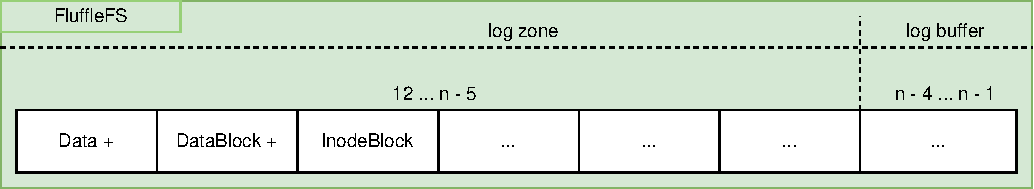
\includegraphics[width=1\textwidth]{resources/images/fluffle-layout-log.pdf}
	\caption{Log zone layout of FluffleFS.}
    % \includesvg[width=0.6\columnwidth]{resources/images/module-dependencies}
    \label{figure:flufflelayoutlog}
\end{figure}

\subsubsection{Memory}

\subsubsection{Operational Rules}

\subsubsection{Concurrency}

\subsection{Offloading}

% Filesystem extended attributes, PID + INODE

\section{Iterations}

This section is covered separetely to prevent clutter in the overall design and
implementation sections. This process consisted of four destinct iterations.
Two relating primarily to the framework, one to the filesystem and one to
offloading. This section describes each iteration briefly before going in more
detail. Firstly regarding framework iterations we see the distinct decision
to switch from a multi process architecture using mmap for shared memory maps to
a monolithic application. The second iteration lead to switching away from the
design of an accelerator API, much like Vulkan \cite{vulkan} or OpenCL, to an
artificial extension of the NVMe namespace. The third iteration changed the use
rtld\_next \cite{rtldnext} to using a practical filesystem with FUSE. Lastly, as
computational storage API our work switched from using
\textit{Portable Operating System Interface} (POSIX) fadvise \cite{fadvise} to
extended attributes.

For each of these four iterations the advantages of the change as well as the
major issues with the previous solution are described. Each iteration is
described in the same order as previously defined.

\subsection{Shared Memory Monolith}

Modern operating systems offer fastly different methods to write sofware. From
kernel modules, to distributed processes, UNIX pipes and shared memory maps.
Choosing the right model impacts practicalities such as the amount of
development effort required and the robustness of the final solution. 
Furtermore, depending on the software architecture some solutions will be better
suited than others.

During the design the use of shared memory maps was replaced with using regular
shared memory. While both solutions provide shared memory they are fundamentally
different. A shared memory map is a file, leveraging the well known UNIX
principle \textit{everything is a file}, that allows two or more processes to
share a region of memory. While regular shared memory is limited to a single
process, however, this memory could be shared across additional threads.

this single process shared memory solution is one of the most common found in
software today. The concepts of such a program are very well understood as
well as the development using imperative languages being straightforward.

While shared memory maps are typically found in device drivers, such as those
for graphics cards, their use consistutes severe additional development effort.
In conjuction with our design being a simulation there is no scientific value in
using shared memory maps for our design. However, for production ready
implementations this decision needs to be reevaluated.

\subsection{NVMe Namespace Command Set}

\subsection{FUSE Filesystem}

% LD\_PRELOAD / RLTD\_NEXT

\subsection{Extended Attributes}

% ---------------------------------------------------------------------------
% ----------------------- end of thesis sub-document ------------------------
% ---------------------------------------------------------------------------